\section{Component view}
\label{sec:component-view}

\begin{figure}
\centering
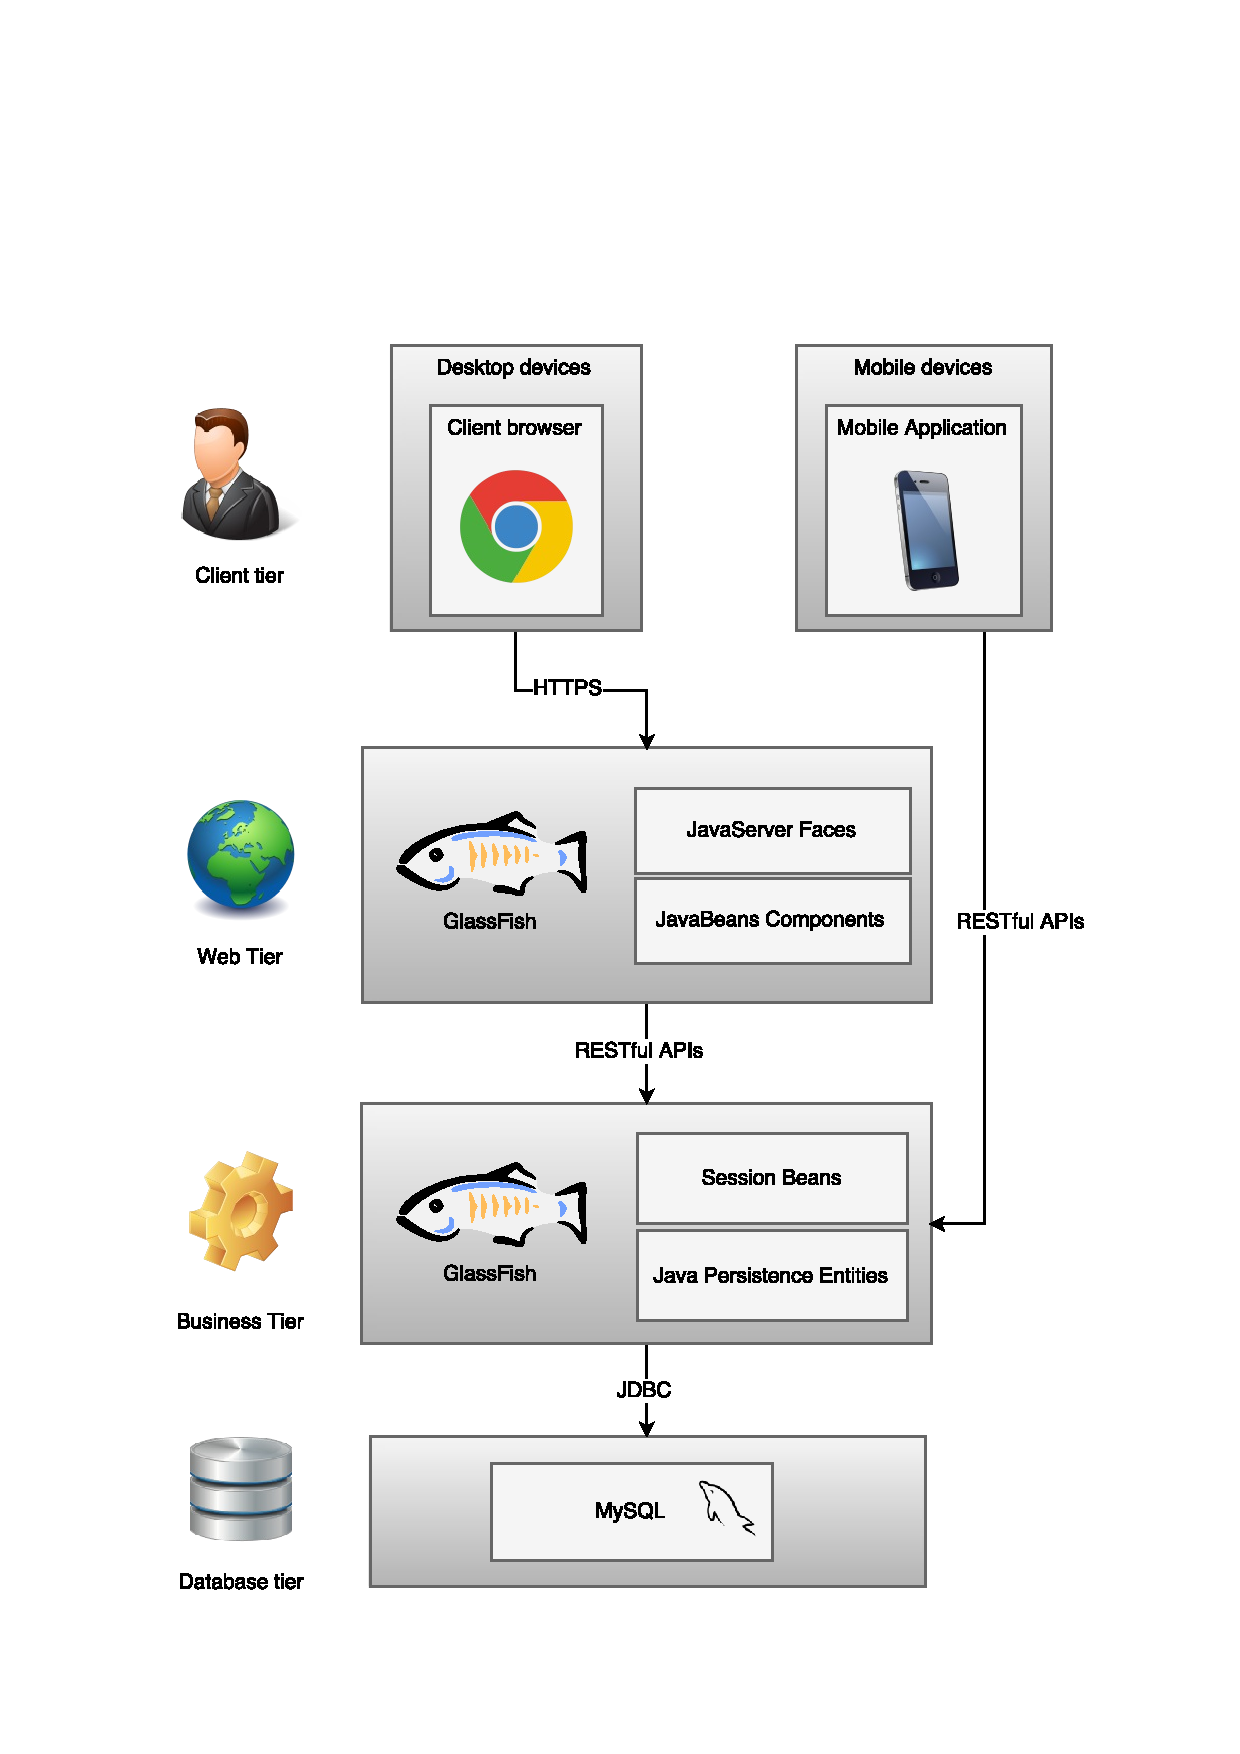
\includegraphics[width=\textwidth]{diagrams/JEE_Tiers}
\caption{The detailed description of tiers, detailed with JEE components.}
\label{fig:tiers-jee}
\end{figure}

\subsection{Database}
The database tier runs MySQL Community Edition and uses InnoDB as the database engine: the DBMS has to support transactions and ensure ACID properties.
The DBMS does not require specific design because it's an external component used as a ``black box'': the database only needs to be configured and tuned in the implementation phase.

The database can communicate only with the business logic tier using the standard network interface, described in \autoref{sec:component-interfaces}.
Security restrictions will be implemented to protect the data from unauthorized access: the database must be physically protected and the communication has to be encrypted. Access to the data must be granted only to authorized users possessing the right credentials. Every software piece that needs to access the DBMS must do so with the minimum level of privilege needed to perform the operations.

All the application data which needs to be persistent is stored in the database. The structure of the tables is illustrated by an E-R diagram. % TODO E-R

Foreign key constraints are used to guarantee some level of data integrity among the tables.
Triggers are not used: the dynamic behaviour of the data is handled entirely by the Java Persistence API in the Business Application tier.

\subsection{Application server}
The application server is implemented in the business logic tier, entirely written in Java EE and run by GlassFish Server.

Access to the database tier is not implemented with direct SQL queries: instead, it's completely wrapped by the \textbf{Java Persistence API (JPA)}. The object-relation mapping is done by entity beans.

The business logic is handled by \textbf{stateless Enterprise JavaBeans (EJB)}.
Our application indeed is rather simple and message-driven: the state of the users is stored in the DB, so we don't need stateful EJB which can be more expensive.
Concurrency management and performance is a great deal for this application, so the reusal of EJBs for many request is a desirable behaviour.

Session Beans used for the application server are shown in~\autoref{fig:session-beans}.
\begin{figure}
    \centering
    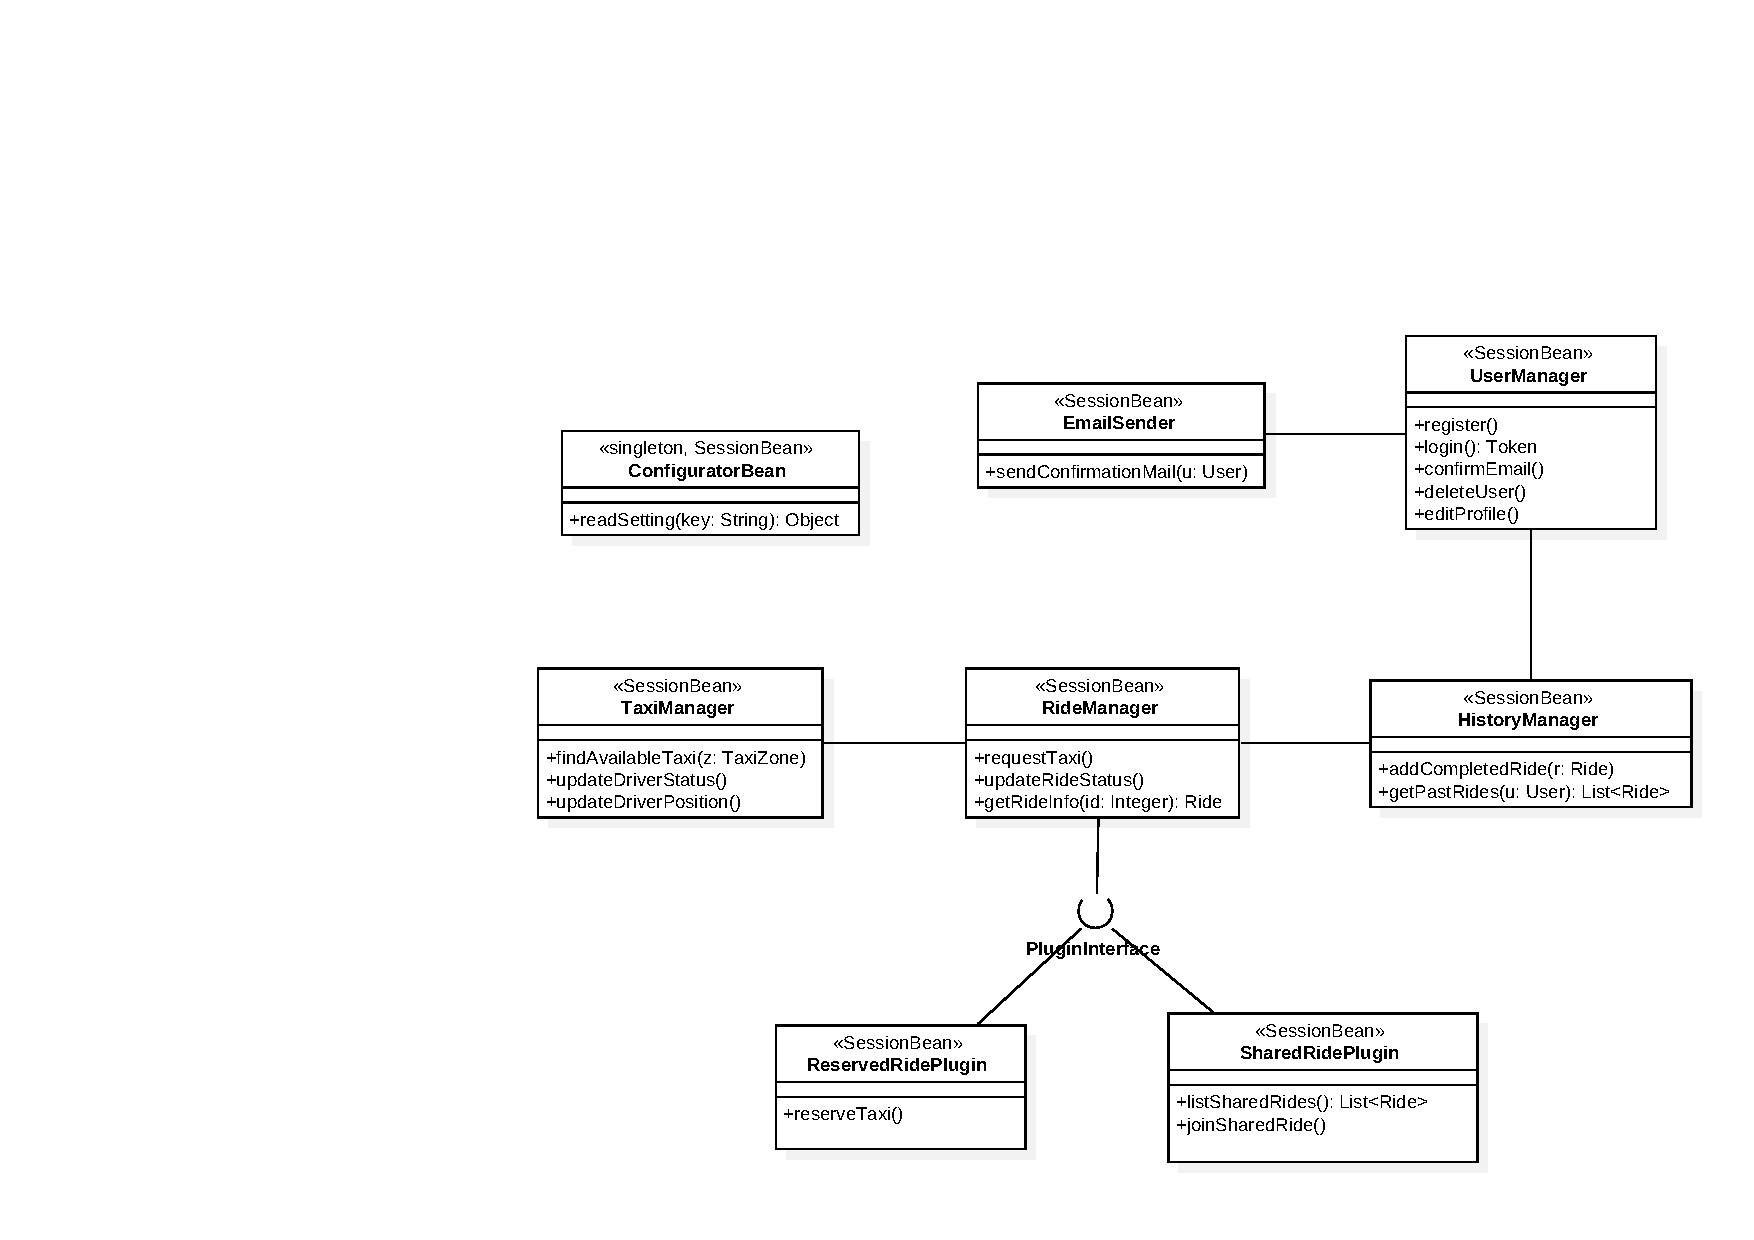
\includegraphics[width=\textwidth]{diagrams/class_sessionbeans}
    \caption{The session beans used in the implementation of the business logic.}
    \label{fig:session-beans}
\end{figure}

The application server implements a RESTful API using JAX-RS to allow the clients (web tier and mobile client) to use the services.

\subsection{Web server}
The web server is implemented using Java EE web components to handle the presentation layer, namely JavaServer Faces (JSF), which is a server-side framework based on MVC.
The web server is run by GlassFish Server.

The web tier only handles the presentation layer: all the business logic is handled by the application server tier. The web tier uses the RESTful interface of the application tier.

Thanks to JSF, the view is written as XML files and is completely separated from the ``application logic'' of the web server. This enables us to write a modular web service.

\subsection{Mobile client}
